\documentclass[a4paper,11pt]{article}
\usepackage[spanish]{babel}
\usepackage[utf8]{inputenc}

% Configuración páginas
\usepackage{vmargin}							% Márgenes

\usepackage{sectsty}							% Fuente de los títulos
\allsectionsfont{\normalfont \Large \scshape}

\usepackage{graphicx}							% Imágenes
\graphicspath{{images/}}

\usepackage{tabularx}							% Otras tablas
\usepackage{listliketab}						% Tratar indentacion distas como tablas

\usepackage{mathtools}							% Matematicas
\newcommand\numberthis{							% numeración en align*
	\addtocounter{equation}{1}\tag{\theequation}
}

\usepackage{algorithm,algpseudocode}			% Algoritmos en latex
\makeatletter
\renewcommand{\ALG@name}{Algoritmo}				% Cambiamos la palabra "Algorithm"
\makeatother
\algnewcommand\Input{\item[\textbf{Entrada:}]}

% Configuración del título
\newcommand{\horrule}[1]{\rule{\linewidth}{#1}} 	% Horizontal rule

\title{
	\vspace{-25pt}
	\normalfont \Large \textsc{
		Modelos de Investigación Operativa,
        Ingeniería Informática\\
        Universidad de Valladolid
	}\\[10pt]
	\horrule{1pt}\\[10pt]
	\huge \textbf{
		Práctica 11
	}\\
	\horrule{1pt}
}
\author{
	\normalfont \Large Daniel González Alonso
}
\date{
	\normalfont \large \today
}

%%%%%%%%%%%%%%%%%%%%%%%%%%%%%%%%%%%%%%%%%%%%%%%%%%
\begin{document}
\maketitle

%%%% RESUMEN %%%%
\begin{abstract}
	En este documento se describen los problemas y los resultados obtenidos de la práctica 11 del tema 5 de la asignatura Modelos de Investigación Operativa de Ingeniería Informática, Universidad de Valladolid.
\end{abstract}

%%%% DESARROLLO %%%%
\section{Introducción}
Esta práctica trata de problemas TSP (\textit{Travelling Salesman Problem}). Los problemas TSP constan de un grafo ${G=(N,A)}$, donde ${N}$ son los nodos del grafo y ${A}$ los arcos entre éstos, con un coste asociado por cada arco, y el objetivo consiste en encontrar el camino Hamiltoniano (un camino que pase por todos los nodos) de coste mínimo.\\

En esta práctica se nos pide implementar la solución al problema TSP con mejora \textit{2-opt}. La mejora \textit{2-opt} en nuestro caso parte de la solución obtenida mediante la heurística del entorno más cercano (explicada en la práctica 10), y pretende mejorarla basándose en que si dos aristas se cruzan, éstas se pueden sustituir por otras de forma que se reduzca la distancia total.\\

Esta sustitución o intercambio se realiza de la siguiente forma: Sean ${\left( i,s\left(i\right) \right)}$ y ${\left( j,s\left(j\right) \right)}$ las aristas a intercambiar, primero sustituirlas por ${\left(i,j\right)}$ y ${\left( s\left(i\right),s\left(j\right) \right)}$. Después invertir la dirección de la ruta existente entre las aristas intercambiadas. La mejora de este intercambio se calcula mediante la siguiente fórmula:

\begin{equation}
\Delta_{i,j} = d\left(i,s(i)\right) + d\left(j,s(j)\right) - d(i,j) - d\left(s(i),s(j)\right)
\end{equation}

%%%%%%%%%%%%%%%%%%%%%%%%%%%%%%%%%%%%%%%%%%%%%%%%%%%%%%
\newpage
\section{Desarrollo}
En esta práctica hay que programar la heurística \textit{2-opt}, a partir de la solución que proporciona la heurística del entorno más cercano, y aplicarlo a los 5 ejemplos de \texttt{n = 21} nodos de las prácticas anteriores y a los 6 problemas Euclídeos.\\\\

Estos problemas se encuentran resueltos mediante \textit{Xpress Mosel} en los ficheros \texttt{tsp \ \_2\_opt\_n21\_1.mos}, \texttt{tsp\_2\_opt\_n21\_2.mos}, \texttt{tsp\_2\_opt\_n21\_3.mos}, \texttt{tsp\_2\_opt\_n21 \ \_4.mos}, \texttt{tsp\_2\_opt\_n21\_5.mos} en el caso de los ficheros \texttt{n21} y por otro lado para los ficheros \texttt{tsp} Euclídeos en los ficheros \texttt{tsp\_2\_opt\_tsp\_60\_1.mos}, \texttt{tsp\_2\_opt\_tsp\_60\_2.mos}, \texttt{tsp\_2\_opt\_tsp \ \_60\_3.mos}, \texttt{tsp\_2\_opt\_tsp\_100\_1.mos}, \texttt{tsp\_2\_opt\_tsp\_100\_2.mos} y \texttt{tsp\_2\_opt\_tsp\_100\_3 \ .mos} (el nombre indica el fichero de datos empleado).\\

Antes de explicar la implementación del algoritmo cabe destacar que los costes ${c_{i,j}}$ en nuestro caso son distancias. Para los ficheros \texttt{n21} la matriz de distancias nos viene dada en el mismo fichero. En el caso de los ficheros \texttt{tsp} solo nos vienen las coordenadas de cada nodo, por ello antes de empezar con estos últimos ficheros hay que calcular la matriz de distancias. Para estos fichero la matriz se calculo mediante la distancia Euclídea redondeada al entero más cercano. En caso de la distancia de un nodo a si mismo, se introducía en esta matriz en vez de 0 un valor ``infinito'' (\texttt{MAX\_INT}).\\

Para la implementación lo primero que hice fue obtener la solución greedy a partir de la heurística del entorno más cercano. Para esto simplemente reutilizé el mismo código que el empleado para la práctica 10, el cual almacenaba la solución en un vector llamado \texttt{siguientes}. Después de obtener la solución greedy, es cuando se aplica la mejora \textit{2-opt} de la siguiente forma:

\begin{enumerate}
\item Buscamos entre los nodos de la solución actual dos nodos ${i}$ y ${j}$ que no sean contiguos y cuya mejora en el caso de que se haga un intercambio ${\Delta_{i,j}}$ sea máximo.

\item Si la mejora entre los nodos a intercambiar es 0, hemos acabado. Si no realizamos el intercambio y volvemos al paso 1.
\end{enumerate}

En mi caso el intercambio lo implementé mediante el siguiente esquema:

\begin{algorithm}[!htbp]
\caption{Intercambio de nodos en \textit{2-opt}}
\label{alg_entorno_cercano}
\begin{algorithmic}[1]
\Input{Nodos $i$ y $j$ a intercambiar y vector con los nodos siguientes $S$}
\State ${S_{2} \gets S}$, ${S(i) \gets j}$, ${S\left( S_{2}(i) \right) \gets S_{2}(j)}$
\State ${k \gets S_{2}(i)}$
\While{${k \neq j}$}
    \State ${l \gets S_{2}(k)}$
    \State ${S(l) \gets S_{2}(k)}$
    \State ${k \gets l}$
\EndWhile
\end{algorithmic}
\end{algorithm}

%%%%%%%%%%%%%%%%%%%%%%%%%%%%%%%%%%%%%%%%%%%%%%%%%%%%%%
\newpage
\section{Resultados}
Los resultados obtenidos para los ficheros de datos de esta práctica fueron los siguientes:

\begin{table}[!htbp]
\label{results_100}
\centering
\begin{tabularx}{\textwidth}{|p{2cm}|X|X|X|X|X|}
\hline
Problema TSP	& \texttt{n21\_1}	& \texttt{n21\_2}	& \texttt{n21\_3}	& \texttt{n21\_4}	& \texttt{n21\_5} \\ \hline
Distancia Total & 213    & 174    & 216    & 189    & 195   \\ \hline
Conexiones  & 1 $\to$ 17 $\to$ 10 $\to$ 20 $\to$ 18 $\to$ 19 $\to$ 13 $\to$ 11 $\to$ 9 $\to$ 12 $\to$ 6 $\to$ 2 $\to$ 16 $\to$ 3 $\to$ 15 $\to$ 8 $\to$ 14 $\to$ 4 $\to$ 7 $\to$ 21 $\to$ 5	& 1 $\to$ 21 $\to$ 13 $\to$ 18 $\to$ 16 $\to$ 11 $\to$ 10 $\to$ 12 $\to$ 17 $\to$ 20 $\to$ 7 $\to$ 6 $\to$ 4 $\to$ 8 $\to$ 9 $\to$ 5 $\to$ 19 $\to$ 3 $\to$ 15 $\to$ 2 $\to$ 14	& 1 $\to$ 7 $\to$ 14 $\to$ 4 $\to$ 21 $\to$ 2 $\to$ 11 $\to$ 9 $\to$ 10 $\to$ 17 $\to$ 5 $\to$ 3 $\to$ 19 $\to$ 12 $\to$ 13 $\to$ 18 $\to$ 8 $\to$ 15 $\to$ 16 $\to$ 20 $\to$ 6	& 1 $\to$ 4 $\to$ 13 $\to$ 21 $\to$ 17 $\to$ 18 $\to$ 19 $\to$ 16 $\to$ 10 $\to$ 8 $\to$ 3 $\to$ 20 $\to$ 9 $\to$ 2 $\to$ 6 $\to$ 7 $\to$ 14 $\to$ 11 $\to$ 15 $\to$ 5 $\to$ 12	& 1 $\to$ 12 $\to$ 14 $\to$ 20 $\to$ 3 $\to$ 6 $\to$ 11 $\to$ 15 $\to$ 5 $\to$ 10 $\to$ 7 $\to$ 16 $\to$ 13 $\to$ 18 $\to$ 9 $\to$ 2 $\to$ 4 $\to$ 19 $\to$ 21 $\to$ 17 $\to$ 8  \\ \hline
\end{tabularx}
\caption{Comparación de los resultados de los ficheros \texttt{n21}}
\end{table}


\begin{table}[!htbp]
\label{results_tsp_60}
\centering
\begin{tabularx}{\textwidth}{|p{2cm}|X|X|X|}
\hline
Problema TSP    & \texttt{tsp\_60\_1}   & \texttt{tsp\_60\_2}   & \texttt{tsp\_60\_3}	\\ \hline
Distancia Total & 680   & 634   & 600   \\ \hline
Conexiones    & 1 $\to$ 28 $\to$ 55 $\to$ 47 $\to$ 43 $\to$ 25 $\to$ 34 $\to$ 16 $\to$ 4 $\to$ 29 $\to$ 18 $\to$ 37 $\to$ 14 $\to$ 13 $\to$ 10 $\to$ 22 $\to$ 60 $\to$ 49 $\to$ 40 $\to$ 39 $\to$ 54 $\to$ 50 $\to$ 31 $\to$ 58 $\to$ 15 $\to$ 26 $\to$ 57 $\to$ 46 $\to$ 6 $\to$ 30 $\to$ 24 $\to$ 41 $\to$ 38 $\to$ 17 $\to$ 2 $\to$ 7 $\to$ 33 $\to$ 3 $\to$ 45 $\to$ 52 $\to$ 19 $\to$ 9 $\to$ 11 $\to$ 44 $\to$ 59 $\to$ 36 $\to$ 56 $\to$ 5 $\to$ 42 $\to$ 48 $\to$ 32 $\to$ 8 $\to$ 12 $\to$ 21 $\to$ 51 $\to$ 20 $\to$ 23 $\to$ 27 $\to$ 53 $\to$ 35	& 1 $\to$ 57 $\to$ 3 $\to$ 36 $\to$ 53 $\to$ 20 $\to$ 2 $\to$ 17 $\to$ 42 $\to$ 48 $\to$ 23 $\to$ 31 $\to$ 41 $\to$ 58 $\to$ 49 $\to$ 59 $\to$ 12 $\to$ 35 $\to$ 11 $\to$ 22 $\to$ 25 $\to$ 19 $\to$ 39 $\to$ 47 $\to$ 14 $\to$ 60 $\to$ 10 $\to$ 24 $\to$ 32 $\to$ 37 $\to$ 15 $\to$ 56 $\to$ 50 $\to$ 40 $\to$ 8 $\to$ 18 $\to$ 51 $\to$ 43 $\to$ 16 $\to$ 21 $\to$ 45 $\to$ 46 $\to$ 52 $\to$ 38 $\to$ 55 $\to$ 6 $\to$ 33 $\to$ 5 $\to$ 27 $\to$ 13 $\to$ 29 $\to$ 44 $\to$ 4 $\to$ 7 $\to$ 54 $\to$ 34 $\to$ 26 $\to$ 28 $\to$ 9 $\to$ 30	& 1 $\to$ 9 $\to$ 58 $\to$ 14 $\to$ 16 $\to$ 44 $\to$ 45 $\to$ 42 $\to$ 17 $\to$ 47 $\to$ 5 $\to$ 55 $\to$ 51 $\to$ 3 $\to$ 19 $\to$ 52 $\to$ 18 $\to$ 56 $\to$ 23 $\to$ 48 $\to$ 59 $\to$ 37 $\to$ 8 $\to$ 36 $\to$ 35 $\to$ 13 $\to$ 32 $\to$ 40 $\to$ 49 $\to$ 38 $\to$ 4 $\to$ 27 $\to$ 50 $\to$ 22 $\to$ 24 $\to$ 31 $\to$ 2 $\to$ 34 $\to$ 57 $\to$ 39 $\to$ 53 $\to$ 29 $\to$ 43 $\to$ 46 $\to$ 33 $\to$ 26 $\to$ 20 $\to$ 28 $\to$ 12 $\to$ 6 $\to$ 41 $\to$ 60 $\to$ 54 $\to$ 15 $\to$ 10 $\to$ 25 $\to$ 11 $\to$ 21 $\to$ 7 $\to$ 30    \\ \hline
\end{tabularx}
\caption{Comparación de los resultados de los ficheros \texttt{tsp\_60}}
\end{table}

\begin{table}[!htbp]
\label{results_tsp_100}
\centering
\begin{tabularx}{\textwidth}{|p{2cm}|X|X|X|}
\hline
Problema TSP    & \texttt{tsp\_100\_1}  & \texttt{tsp\_100\_2}  & \texttt{tsp\_100\_3}  \\ \hline
Distancia Total & 777    & 793   & 827   \\ \hline
Conexiones	& 1 $\to$ 51 $\to$ 30 $\to$ 56 $\to$ 55 $\to$ 9 $\to$ 15 $\to$ 28 $\to$ 86 $\to$ 27 $\to$ 29 $\to$ 92 $\to$ 48 $\to$ 11 $\to$ 13 $\to$ 95 $\to$ 49 $\to$ 76 $\to$ 78 $\to$ 5 $\to$ 69 $\to$ 20 $\to$ 43 $\to$ 35 $\to$ 54 $\to$ 58 $\to$ 89 $\to$ 21 $\to$ 87 $\to$ 91 $\to$ 68 $\to$ 34 $\to$ 7 $\to$ 22 $\to$ 90 $\to$ 62 $\to$ 44 $\to$ 94 $\to$ 70 $\to$ 85 $\to$ 96 $\to$ 88 $\to$ 38 $\to$ 60 $\to$ 77 $\to$ 14 $\to$ 83 $\to$ 37 $\to$ 46 $\to$ 84 $\to$ 26 $\to$ 8 $\to$ 98 $\to$ 61 $\to$ 16 $\to$ 42 $\to$ 12 $\to$ 66 $\to$ 52 $\to$ 32 $\to$ 53 $\to$ 72 $\to$ 17 $\to$ 25 $\to$ 10 $\to$ 71 $\to$ 23 $\to$ 65 $\to$ 18 $\to$ 74 $\to$ 6 $\to$ 75 $\to$ 73 $\to$ 3 $\to$ 100 $\to$ 33 $\to$ 39 $\to$ 81 $\to$ 97 $\to$ 45 $\to$ 19 $\to$ 82 $\to$ 67 $\to$ 79 $\to$ 2 $\to$ 50 $\to$ 93 $\to$ 4 $\to$ 99 $\to$ 47 $\to$ 36 $\to$ 63 $\to$ 80 $\to$ 64 $\to$ 31 $\to$ 40 $\to$ 57 $\to$ 59 $\to$ 24 $\to$ 41	& 1 $\to$ 87 $\to$ 20 $\to$ 31 $\to$ 16 $\to$ 23 $\to$ 76 $\to$ 63 $\to$ 72 $\to$ 29 $\to$ 58 $\to$ 10 $\to$ 17 $\to$ 30 $\to$ 36 $\to$ 90 $\to$ 15 $\to$ 60 $\to$ 83 $\to$ 64 $\to$ 7 $\to$ 40 $\to$ 74 $\to$ 19 $\to$ 43 $\to$ 66 $\to$ 73 $\to$ 79 $\to$ 80 $\to$ 93 $\to$ 50 $\to$ 3 $\to$ 32 $\to$ 85 $\to$ 61 $\to$ 25 $\to$ 99 $\to$ 38 $\to$ 12 $\to$ 2 $\to$ 95 $\to$ 49 $\to$ 46 $\to$ 69 $\to$ 100 $\to$ 41 $\to$ 91 $\to$ 88 $\to$ 70 $\to$ 18 $\to$ 33 $\to$ 98 $\to$ 78 $\to$ 77 $\to$ 86 $\to$ 9 $\to$ 5 $\to$ 8 $\to$ 57 $\to$ 59 $\to$ 6 $\to$ 55 $\to$ 53 $\to$ 51 $\to$ 26 $\to$ 21 $\to$ 13 $\to$ 81 $\to$ 82 $\to$ 45 $\to$ 22 $\to$ 65 $\to$ 14 $\to$ 4 $\to$ 35 $\to$ 92 $\to$ 62 $\to$ 11 $\to$ 84 $\to$ 24 $\to$ 34 $\to$ 39 $\to$ 54 $\to$ 67 $\to$ 47 $\to$ 75 $\to$ 27 $\to$ 37 $\to$ 56 $\to$ 68 $\to$ 42 $\to$ 94 $\to$ 48 $\to$ 44 $\to$ 71 $\to$ 97 $\to$ 89 $\to$ 52 $\to$ 96 $\to$ 28	& 1 $\to$ 16 $\to$ 60 $\to$ 22 $\to$ 71 $\to$ 46 $\to$ 95 $\to$ 100 $\to$ 19 $\to$ 69 $\to$ 98 $\to$ 23 $\to$ 20 $\to$ 4 $\to$ 42 $\to$ 72 $\to$ 2 $\to$ 31 $\to$ 50 $\to$ 8 $\to$ 9 $\to$ 59 $\to$ 87 $\to$ 43 $\to$ 5 $\to$ 32 $\to$ 53 $\to$ 11 $\to$ 85 $\to$ 86 $\to$ 12 $\to$ 10 $\to$ 94 $\to$ 66 $\to$ 99 $\to$ 55 $\to$ 18 $\to$ 57 $\to$ 51 $\to$ 76 $\to$ 91 $\to$ 74 $\to$ 65 $\to$ 29 $\to$ 33 $\to$ 36 $\to$ 79 $\to$ 44 $\to$ 38 $\to$ 82 $\to$ 28 $\to$ 56 $\to$ 52 $\to$ 13 $\to$ 54 $\to$ 48 $\to$ 40 $\to$ 81 $\to$ 89 $\to$ 84 $\to$ 41 $\to$ 75 $\to$ 47 $\to$ 24 $\to$ 6 $\to$ 64 $\to$ 26 $\to$ 15 $\to$ 77 $\to$ 61 $\to$ 35 $\to$ 37 $\to$ 83 $\to$ 27 $\to$ 58 $\to$ 80 $\to$ 39 $\to$ 17 $\to$ 70 $\to$ 62 $\to$ 7 $\to$ 78 $\to$ 3 $\to$ 45 $\to$ 96 $\to$ 14 $\to$ 92 $\to$ 63 $\to$ 34 $\to$ 73 $\to$ 97 $\to$ 21 $\to$ 25 $\to$ 30 $\to$ 90 $\to$ 68 $\to$ 67 $\to$ 88 $\to$ 93 $\to$ 49	\\ \hline
\end{tabularx}
\caption{Comparación de los resultados de los ficheros \texttt{tsp\_100}}
\end{table}

\newpage{2}
También obtuve los gráficos IVE para los ficheros \texttt{tsp}. En este caso aquí se muestra el resultado obtenido para el fichero \texttt{tsp\_100\_1}:

\begin{figure}[!htbp]
	\centering
	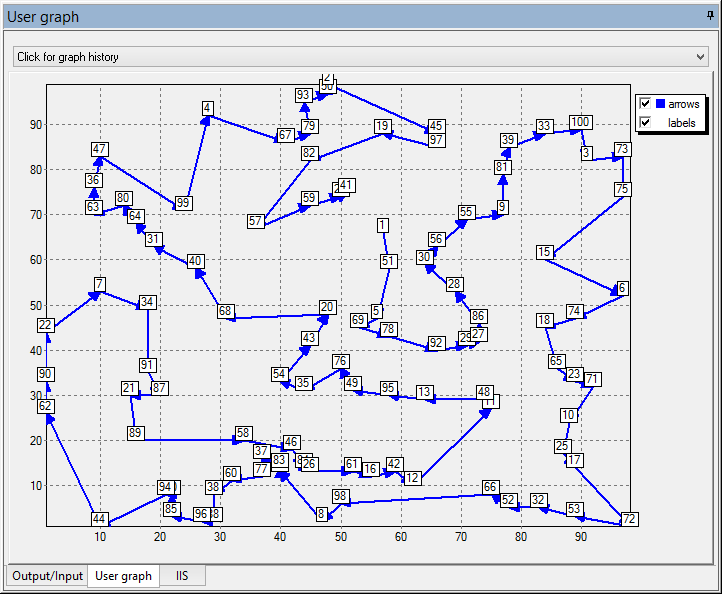
\includegraphics[width=1.0\textwidth]{2opt_100_1.png}
\end{figure}

\end{document}
